%!TEX root = ./main.tex

\renewcommand{\inPoints}{}

\pgfmathsetmacro\pointsPerLine{4}% in [1,\infty[
\newsavebox\geometrya
\sbox{\geometrya}{%
	\pgfmathsetmacro\dimension{1}% in [0,3]
	\input{figures/geometry_print}%
}
\newsavebox\geometryb
\sbox{\geometryb}{%
	\pgfmathsetmacro\dimension{2}% in [0,3]
	\input{figures/geometry_print}%
}
\newsavebox\geometryc
\sbox{\geometryc}{%
	\pgfmathsetmacro\dimension{3}% in [0,3]
	\input{figures/geometry_print}%
}

\begin{frame}
	\begin{minipage}{\textwidth}
		\centering%
		$S_k(3) = \underbrace{PG(1,3) \otimes \dots \otimes PG(1,3)}_{k\text{ times}}$
	\end{minipage}
	\resizebox{\textwidth}{!}{
		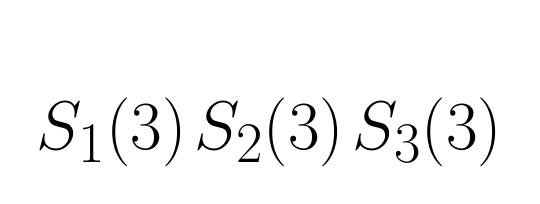
\begin{tikzpicture}
			\uncover<2->{
				\node (geometrya) at (0,0) {\usebox{\geometrya}};
				\node[anchor=north,yshift=-15,font=\Huge] at (geometrya.south) {$S_1(3)$};
			}
			\uncover<3->{
				\node[anchor=south west, xshift=50] (geometryb) at (geometrya.south east) {\usebox{\geometryb}};
				\node[anchor=north,yshift=-15,font=\Huge] at (geometryb.south) {$S_2(3)$};
			}
			\uncover<4->{
				\node[anchor=south west, xshift=50] (geometryc) at (geometryb.south east) {\usebox{\geometryc}};
				\node[anchor=north,yshift=-15,font=\Huge] at (geometryc.south) {$S_3(3)$};
			}
		\end{tikzpicture}
	}
	\begin{tikzpicture}[remember picture,overlay,x={(1pt,0pt)},y={(0pt,1pt)}]
		\node[anchor=south east] at ($(current page.south east)+(-3,10)$) {\tiny\textit{S stands for Segre varieties}};
	\end{tikzpicture}
\end{frame}
